\documentclass[a4paper, 10pt, dvipdfmx]{jlreq}

\usepackage{amsmath,amsfonts,amssymb}
\usepackage{bm}
\usepackage{mathtools}
\usepackage{siunitx}
\usepackage[dvipdfmx]{graphicx}
\usepackage[dvipdfmx]{color}
\usepackage[dvipdfmx, colorlinks=true, allcolors=blue]{hyperref}
\usepackage{listings}
\usepackage{tikz}
\usepackage{physics}
\usepackage{url}

\Urlmuskip=0mu plus 10mu
\allowdisplaybreaks[4]
\frenchspacing
\definecolor{OliveGreen}{rgb}{0.0,0.6,0.0}
\definecolor{Orange}{rgb}{0.89,0.55,0}
\definecolor{SkyBlue}{rgb}{0.28, 0.28, 0.95}
\lstset{
  language={c++},
  basicstyle={\ttfamily},
  identifierstyle={\small},
  ndkeywordstyle={\small},
  frame=single,
  breaklines=true,
  numbers=left,
  xrightmargin=0zw,
  xleftmargin=3zw,
  numberstyle={\scriptsize},
  lineskip=-0.9ex,
  keywordstyle={\small\bfseries\color{SkyBlue}},  
  commentstyle={\color{OliveGreen}}, 
  stringstyle={\small\ttfamily\color{Orange}}    
}

\begin{document}

\title{2012年度 大問2}
\author{hari64boli64 (hari64boli64@gmail.com)}
\date{\today}
\maketitle

\section{問題}

線形回帰モデル

\section{解答}

\subsection*{(1)}

\begin{equation*}
  \hat{\beta}=(X^\top X)^{-1}X^\top y
\end{equation*}

\subsection*{(2)}

\begin{equation*}
  \mathbb{E}[\hat{\beta}] =\beta
\end{equation*}

\subsection*{(3)}

\begin{equation*}
  \Sigma=\sigma^2(X^\top X)^{-1}
\end{equation*}

\subsection*{(4)}

\begin{equation*}
  \mathbb{E}[(y_{n+1}-x_{n+1}^\top \beta)^2]=\sigma^2\qty(1+x_{n+1}^\top (X^\top X)^{-1}x_{n+1})
\end{equation*}

\section{おまけ}

\lstinputlisting[caption=problem4,label=code:problem4,language=Python]{2.py}

\begin{figure}[htbp]
  \begin{center}
    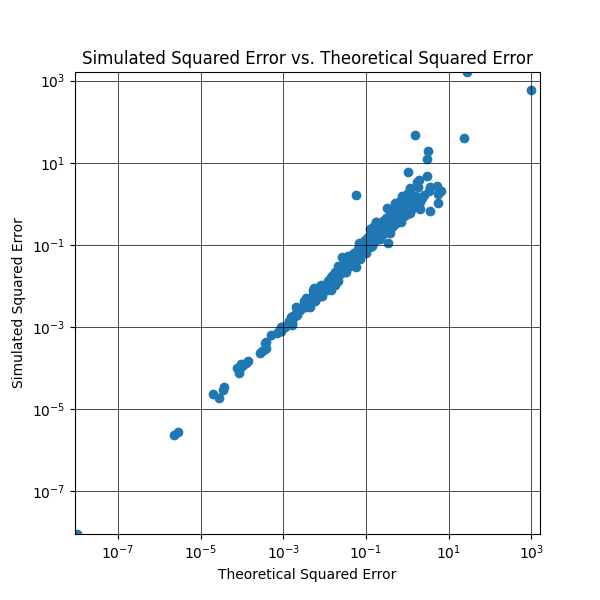
\includegraphics[height=80mm]{2.png}
    \caption{問題4のグラフ (シミュレーション値と理論値)}
  \end{center}
\end{figure}

\end{document}
